\section{Hash function}
An hash function is a function that converts a binary string of arbitrary length to a binary string of fixed length.
The length count s in bits and normally has a huge maximum length in input (zero length is permitted as well) and the output is of fixed length, usually in the set 128, 160, 256, 512.

Usually the more the output length, the more it is difficult to have a collision.

\subsection{Non crypto hash}
There are various crypto functions for which it is easy to compute a collision, those ones are not secure, they are not suitable for security application.

Non crypto hash can of course be useful for other application like error detection, as the CRC or XOR.
They are useful because a random error in transmission will unlikely yield a collision, moreover they are fast to compute.

NB: some non crypto hashes have been used for security purposes with various problems, for example the WEP WiFi protocol used CRC and so it is easy to compute WiFi credentials.

\subsection{Crypto hash}
The key point of cryptographic hashes is in the difficulty of finding a collision, not it's impossibility.

The maximum number of guesses to certainly find a collision by a brute force approach is of course $2^{256}+1$ distinct attempts for a 256 bit length hash.
However it is possible to show that a collision can be found with high probability long before the exhaustive approach.
Basically we have $50\%$ of probability of a collision after $2^{128}$, as a general rule roughly the square root of the number of possible output.
This is true using $O(2^{\frac{n}{2}})$ time and space (with $n = len(H)$).

\subsubsection{Birthday paradox}
This is an interesting result of birthday paradox: with $n$ people in a room how large should be $n$ before the probability that two of them share a birthday becomes larger than $50\%$?
Since a year is made of 365 days and all days are equally probable we have as a result that with $n = 23 \approx \sqrt{365}$ two people will share a birthday with probability just above $50\%$.

Let's try to understand why:
\begin{itemize}
    \item let's take a room with a single person, when introducing another one in order to not match the birthday of the first one we have 364 possible birthdays, so 
$$
    \frac{364}{365} = 0.9973
$$
    \item when a third person enters the room it has to avoid two birthdays, in order to get the probability that none of them share a birthday we have a probability of:
$$
    \frac{364}{365} \cdot \frac{363}{365} = 0.9918
$$
    \item when we have 9 people in the room the probability that everyone avoid each other birthday has dropped to $90\%$ and the opposite condition of having at least a pair of people that shares a birthday has raised to $10\%$.

    \item in the end when the $23^{th}$ person enters the room, the chance of each one having a unique birthday has dropped to $0.49\%$, and so the chance that at least two people share a birthday is now above $50\%$.
\end{itemize}

\subsubsection{Adversarial collision resistance}
Common hash functions minimize the chance of collision f the inputs are chosen at random but if an adversary is specifcally looking for a collision, it is easy to find it.

Adversarial collision resistance means that for an adversary it must be difficult to find a collision.

\subsubsection{One way}
A cryptographic hash should be one way: it should be easy and efficient to obtain an hash from an input but at the same time it should be difficult to invert, so recover the input who produces a specific hash.

This property is also called \emph{preimage resistance}: for any $y \in Y$, it is hard to find $x \in X$ such that $h(x) = y$. 

There exists also the \emph{second preimage resistance}: given $M$ and thus $h(M)$ it is hard to find another $M'$ such that $h(M') = h$.
It is also called \emph{weak collision resistance}. 

\subsubsection{Avalanche effect}
A small change in the input should produce a completely different output.

\subsubsection{Hiding}
Suppose that an application just tosses a coin and returns this result:
$$
    H_{toss}(outcome) = (1+outcome) mod 2
$$
then we have: $H_{toss}(Heads) = 1$ and $H_{toss}(Tail) = 0$.

In this scenario if the attacker is able to find the domain $\{Heads, Tail\}$, once it sees the outcome it can try hashing each value of the domain and understand the toss outcome.

The main problem here is that the input domain is easily enumerable.
The \emph{hiding} property is related to the preimage property!

As a solution we can:
\begin{itemize}
    \item pick a random integer $R$, for example of 256 bits, from a distribution with a \emph{high min entropy} (every value in the distribution are equally likely to be chosen)

    \item append $R$ to the original input;

    \item the input space now becomes extremely hard to enumerate (since we have now $2^{257}$ bits of input size).
\end{itemize}

We can define the hiding property as: a hash function $H$ is said to be \emph{hiding} if when a secret value $R$ is chosen from a probability distribution that has high min-entropy, then, given $H(R || x)$ it is infeasible to find $x$.

\subsection{Attacking hash functions}
The usual approach for attacking an hash function relies on exploiting logical weaknesses in the algorithm or on how the hash is used inside the application.
Of course there is still the brute-force attack (the exhaustive search).

\subsection{Use of cryptographic hash}
Cryptographic hashes are used:
\begin{itemize}
    \item to show commitment: for example in auctions we can bid a certain prize without openly revealing the value to all and only later reveal the value;
    \item hash puzzle: for example hashes is used as a proof or work in Bitcoin;
    \item hash pointer: an hash can be used as a pointer to a unique reference;
    \item much more.
\end{itemize}

\subsubsection{Commitment scheme}
Let's suppose that Alice and Bob wants to play paper-scissors-stone over the telephone (or internet) without trusted third party.
We want a fair game so no one decides his/her choice after acquiring the other's choice, but this is only possible if they express their choices together, which is unlikely in the internet/mobile call context.

We can develop a commitment scheme: basically we seal our choice in an envelope and put that envelope out on the table where everyone can see it, of course we can't change the value which is inside.
At the end of the bets we can open the envelope and reveal the actual value.

\begin{verbatim}
    Commit phase: P computes and sends com to V:
        r = random()
        com = commit(secret, r)

    Open phase:
        P reveals secret and r to V:
        V verifies commit(secret, r) == com
\end{verbatim}
The commit phase is also called \emph{hiding} while the open phase is also called \emph{binding}.

In the example of the paper-scissor-stone we can develop the following scheme:
\begin{itemize}
    \item Alice commits to her choice by generating a random number $RA$ and computing and sharing $h_A = h(RA || paper)$
    \item Bob then can make his choice but can't know what Alice committed to;
    \item at the end Alice reveals it's choice: $paper$ and it's secret value: $RA$ which can be validated by Bob in order to acknowledge his lose/win.
\end{itemize}
In this scheme Bob can understand if Alice cheated because the first hash is not equal to the one generated with the public revealed data.

\subsubsection{Search puzzles}
Ah hash/search puzzle consists of:
\begin{itemize}
    \item a cryptographic hash function $H$;
    \item a random value $r$;
    \item a target set, $S$;
    \item a solution of the puzzle is a value $x$ such that: $m = r || x$ and $H(m) \in S$
\end{itemize}
This search is based on partial pre-image attack because we have to find a part of the input such that the output belongs to a set.

Bitcoin proof-of-work is based on a hash/search puzzle.
By enlarging or restricting the subset we can tune the difficulty of the puzzle, Bitcoin network uses this in order to have always the same time to solve the puzzle independently from the size of the network.

\subsection{Puzzle-friendliness property}
A hash function $H$ is said to be puzzle-friendly if: for every possible $n$-bit output value $y$, if $k$ is chosen from a distribution with high min-entropy then it is infeasible to find $x$ such that $H(k || x) = y$ in time significantly less than $2^n$.

This property implies that: there is no solving strategy to solve a search puzzle that is much better than trying exaustively all the values of $x$.

\subsection{Some more usages}
\begin{itemize}
    \item Digital signatures;
    \item deduplication;
    \item password storage.
\end{itemize}
Basically hash functions can be used to generate \emph{data fingerprint}: if we know that $H(x) = H(y)$ it is safe to assume that $x = y$ because it is unlikely to have a collision, but it's easier to compare a small value instead of the whole file.
Based on that fingerprint we can to deduplication avoiding to store different files who have the same hash, we can do antitampering checking that the hash is still the same as before uploading/downloading, etc.

Moreover Bitcoin uses block chain (which is an hash chain) to store transaction ledger in a p2p network building a tamper freenes property.

\section{Digital signature}
\subsection{Public key cryptography}
Digital signature is based on public-key cryptography which are asymmetric encryption algorithm.
We have two different keys instead of one:
\begin{itemize}
    \item a public key: publicly known by everyone;
    \item a private one: only known by the owner.
\end{itemize}
What a key encrypts the other can decrypt, and viceversa.

\subsubsection{Confidentiality}
A public-key cryptography scheme can produce confidentiality:
\begin{itemize}
    \item Alice wants to send a message to Bob, so encrypts the message $m$ with the public key of Bob and sends the result to it;
    \item Bob then can use it's private key to decrypt and read the message from Alice.
\end{itemize}
There is no way to decrypt the message not having the private key of Bob, but everyone can encrypt messages.

Moreover there is no need to agree on a common key for both sender and receiver.

Another key feature of this cryptographic scheme is tat it is relatively easy to compute the public key from the private key but it should be hard to compute the private one from the public key, which is of course publicky known.

\subsection{Integrity}
A digital signature can produce integrity (autheticity) of the message:
\begin{itemize}
    \item we get a message $m$;
    \item we compute the hash of $m$;
    \item we encrypt the hash of the message with out \emph{private} key;
    \item we send the message along side the encrypted hash.
\end{itemize}
If the receiver then wants to verify the received message, then it can:
\begin{itemize}
    \item read the message and hash it;
    \item use the public key of the sender in order to decrypt the received hash;
    \item check for equality between the computed hash and thee decrypted one.
\end{itemize}
If the message has been modified during the transmission then the computer hash would be different from the decrypted one, and it is unfeasible to get an actual encrypted hash for someone who doesn't know the private key of the sender.

NB: this scheme doesn't guarantee confidentiality since the message is still sent in clear, alongside the integrity hash.

\subsubsection{APIs for digital signature}
\begin{verbatim}
    (sk, pk) = generateKeys(keysize)
        // sk: secret (private) key, used for signing
        // pk: public key, used for verification

    sig := sign(sk, message)
        // hash the message and encrypt the hash
    isValid := verify(pk, message, sig)
        // decrypt the signature and compare
        // the result with the hashed message
\end{verbatim}
The following property must hold:
$$
    verify(pk, message, sign(sk, message)) == true
$$

\subsection{Construction}
There are various digital signature schemes, all of them based on a one way trapdoor function.
The most famous example is the one made from the RSA algorithm which is based on the factorization problem.

There is also the DSA scheme based on the discrete logarithm and the ECDSA (used in Bitcoin) which is a variant of DSA over elliptic curves.


\section{Hash pointer}
An hash pointer is a pointer to where some infos is stored with a cryptographic hash of the info.
Given an hash pointer we can have two primitives:
\begin{itemize}
    \item ask to get the info back, by following the pointer;
    \item verify that info associated to the pointer are not changed.
\end{itemize}

This concept is the basic structure used in building the blockchain, which is basically a list linked with hash pointers:
\begin{figure}[H]
    \centering
    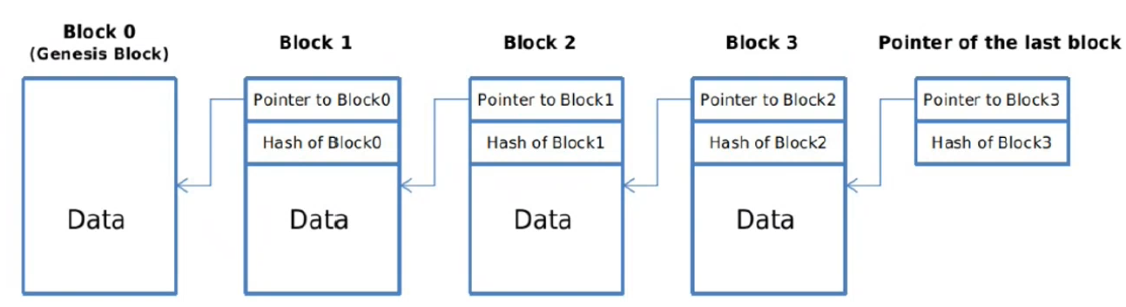
\includegraphics[width=250px]{images/4_Cryptographic_Toolbox/01.png}
    \caption{Blockchain}
\end{figure}

The principal use case of this structure is the tamper-evident log, a basic structure in blockchain, because if something changes in one block, then the hashf of the next block will not match up, obviously because the has is collision resistant.
Moreover in PoW-based blockchain, the single block contains also the proof that PoW has been succesfully executed ,so if data is changed, then the PoW has to be re-executed for all the blocks which is computationally infeasible.

In general hash pointers can be used in any pointer-based data structure that has no cycles (directed, acyclic graphs).

\section{Bloom filters}
Consider having a set $S = \{ s_1, s_2, ..., s_n \}$ of $n$ elements with $n$ very large and we want an efficient data structure supporting membership queries.
We can build a succint data structure to implement an approximated solution to the set membership problem.
Whit this data structure we can have false positive but we can also decide a trade off between space required to implement the structure and the probability of false positives.

In order to build a bloom filter we take a binary vector $S$ of $m$ bits, initially set to 0, then we decide $k$ hash functions (not necessarily cryptographic ones).
In order to insert an element $x$ in the structure we compute the various $h_{i}(x) \forall i = 1, ..., k$ and set to 1 the corresponding $S [h_{i}(x) ] $.

To have a good structure we usually build $m > n \cdot k$, with each hash function that returns uniformly distributed in the range $[1, m]$.

To look up for an element in the bloom filter we re-hash the key we are searching for and check if each obtained position is to 1, if it's not then we are sure that the element is not present in the structure, otherwise if all interested positions are set to 1 then there is the possibility that the element we are looking for is present inside the structure.

\subsection{Probability of false positive}
The probability that, after all $n$ elements are mapped to the vector, a specific bit of the filter (of size $m$) has still value 0 is:
$$
    p' = \left( 1 - 1/m \right)^{kn} \approx e^{\frac{-kn}{m}}
$$
(approximation derived from the definition of $e$).
This value is also the percentage of bits set to 0 after the full construction.

Considering an element that does not belong to the set and applying the $k$ functions a false positive is obtained if all the $k$ hash functions return a value of 1 and the probability of this event is:
$$
    \left( 1 - e^{\frac{-kn}{m}} \right)^k
$$
so we have that the probability of false positive depends both on:
\begin{itemize}
    \item the ratio $\frac{m}{n}$: the number of bits for each element of the set;
    \item $k$: the number of hash functions.
\end{itemize}

Fixing the ratio it seems that two conflicting factors for defining $k$ exists:
\begin{itemize}
    \item decreasing $k$ increases the number of 0 and with it the probability to have a false positive should decrease;
    \item increasing $k$ increases the precision of the method and with that the probability of false positive should decrease as well.
\end{itemize}

Fixing instead $k$ the probability of false positives exponentially decreases when $m$ increases, moreover for low values of $\frac{m}{n}$ the probability is higher for large values of $k$.

A bloom filter becomes effective when $m = c \cdot n$ with $c$ constant value.

\subsection{Operations}
\subsubsection{Union}
To compute the union between two bloom filters $B_1$ and $B_2$ having the same size and the same hashing functions we need to bitwise OR the two.

\subsubsection{Deletion}
It is not possible to delete entries in the bloom filter because of the conflicts.
However there is a variant of this data structure named counting bloom filters (spectral bloom filters) in which each entry is a counter instead of a single bit, so we can:
\begin{itemize}
    \item at insertion time we just increment the counters indexed by the hash results;
    \item at deletion time we decrease the counter.
\end{itemize}

\subsubsection{Intersection}
To compute the intersection between two bloom filters $B_1$ and $B_2$ having the same size and the same hashing functions we need to bitwise AND the two.
Of course we obtain an approximation because that single bit could be set to 1 by different values in the two sets that does not necessarily appears in the actual intersection.

\subsection{Usages}
A bloom filter is used in bitcoin in order to build a lightweight mobile nodes.
Since those nodes have constraints on memory and power they send a bloom filter, populated with the Bitcoin addresses they are interested into, to a full Bitcoin client, then when the full node receives a block $B$ of the blockchain, it can check the BF in order to decide whether to inform the lightweight node or not.

In Ethereum instead it is used to summarize events generated by smart contracts, for example to find all the tokens sold by a specific user in a block of 500 transactions instead of parsing all the transactions we can query a bloom filter in the header of a block for the presence of that users and perform a search in the block only if a match is found.

There are of course also usages not related to blockchain, for example in the database search to avoid useless disk lookup we can use a bloom filter and only if there is the possibility of a match going through the actual retrieve.

\section{Merkle hash tree}
A merkle hash tree is a data structure introduced by Ralph Merkle in 1979 used to summarize a big quantity of data with the goal of verifying the correctness of the content.
It's based on a complete binary tree of hashes built starting from an initial set of data and then:
\begin{itemize}
    \item the $i$-th leaf stores the hash $h_i$ of the value $f_i$;
    \item an internal node contains the hash of the concatenation of the hashes of its sons;
    \item the last hash stored in the root is called Merkle Root hash.
\end{itemize}
\begin{figure}[H]
    \centering
    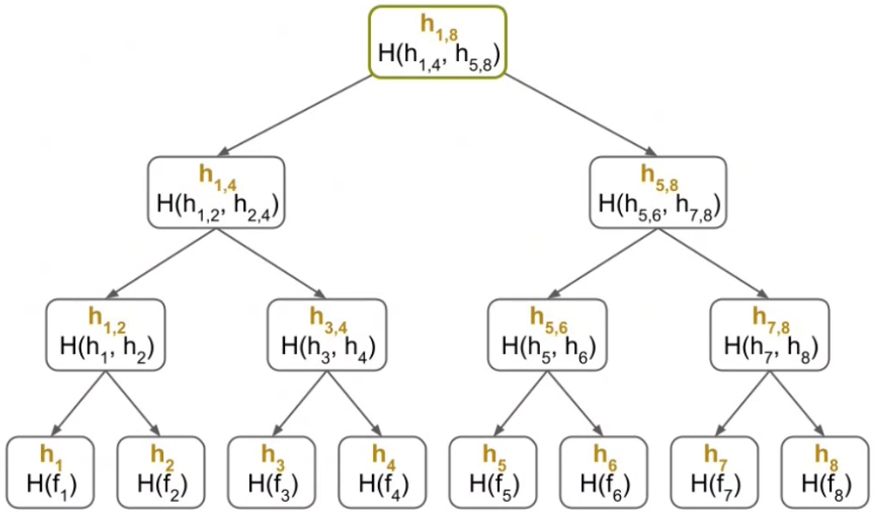
\includegraphics[width=300px]{images/4_Cryptographic_Toolbox/02.png}
    \caption{Merkle tree structure}
\end{figure}

In order to build a working Merkle tree we need a collision-resistant hash function, so basically a cryptographic hash.

\subsection{Merkle proof}
Let's suppose that Alice (verifier) only knows the Merkle root hash $h$, Bob (the prover) can give Alice one of the values $x_i$ and convince Alice that actually it is the $i$-th value used to build the tree.
To convince her Bob can give an associated Merkle proof without showing all the other inputs.

With a merkle proof that says that $x_i$ was the $i$-th input used to compute $h$, no attacker can come up with another Merkle proof that says that a differet $x' \neq x_i$ was the $i$-th input used for that tree. 

\subsection{Merkle proof}
A Merkle proof contains the subset of hashes of the Merkle tree, that, together to the single leaf allow to recompute the root hash, basically the siblings of all the nodes on the path from the specific leaf to the root.
To verify the proof all we have to do is to actually compute the hashes on the path and check whether the result is equal to the known root hash.

\subsection{Consistency}
It is unfeasible to output a Merkle root $h$ and two inconsistent proof $\Pi_i$ and $\Pi'_i$ for two different inputs $x_i$ and $x'_i$ at the $i$-th leaf in the tree of rize $n$.
The proof can be done by intuition:
\begin{itemize}
    \item if the Merkle proof is verified, you were able to recompute the root hash by using $f_i$ as the $i$-th and the Merkle proof as the remaining inputs;
    \item if the proof verification had yielded the same hash but with a different file $f'_i \neq f_i$ as the $i$-th input, this would yield a collision in the underlying hash function $H$ used to build the tree, which is not possible if $H$ is collision resistant.
\end{itemize}

\subsection{Why use a merkle tree}
We could think about storing the hash of each of the files to check their integrity, and then just check the hash of the single file to be sure of its integrity.
However a merkle tree is thought to scale to billions of files and allows to compute check in $O(log n)$.

\section{Trie}
A trie is a data structure for applications performing extensive string processing and retrieval operations, mainly for search engines and natural language processing.
It's a tree-like data structure in which:
\begin{itemize}
    \item the root node stores nothing;
    \item edges are labeled with letters and a path from the root to the node represents a string;
    \item the nodes come with an indicator which indicates whether that node represents the end of a string.
\end{itemize}

Every node, except the root node represents a prefix of a string in fact it is called also \emph{prefix-tree}.

\subsection{Patricia trie}
The trie representation requires high space because the majority of nodes have just one child.
It is possible to compress the trie by combining nodes with just one child into a complete substring on the path, instead of a single character.
This is the basic idea behind a \emph{patricia trie}.

NB: Patricia stands for Practical Algorithm To Retrieve Information Coded In Alphanumeric.

\subsection{Patricial Merkle trie}
A Patricia Merkle trie is the combination of:
\begin{itemize}
    \item Patricia trie: to enable faster search of data and store keys while grouping their common path in a node;
    \item Merkle trie: to maintain data integrity and tamper proof validation.
\end{itemize}
It's a new data structure introduced in the yellow paper of Ethereum used to represent the state of the accounts and smart contracts, and now used in most EVM-based blockchains.

It's organized as a tree with every node hashed in the sense of Merkle proof grouping common paths in the sense of Patricia tries.
Moreover tries can be used to represent key-value pairs:
\begin{itemize}
    \item use the key to take the right path;
    \item then store the associated value in the node which is the end of the path.
\end{itemize}

\subsubsection{Structure}
A merkle patricia trie can have three type of nodes:
\begin{itemize}
    \item branch node: a node that has more than one child node, it stores links to child nodes and may store a value too;
    \item extension node: a non-leaf node representing a sequence of nodes that has only one child.
    It's basically a compression node for a full path of only one child nodes.
    It stores a key value that represents the combined nodes and a link to the next node;
    \item leaf node (value node): similar to extension node but stores a value.
\end{itemize}

\begin{figure}[H]
    \centering
    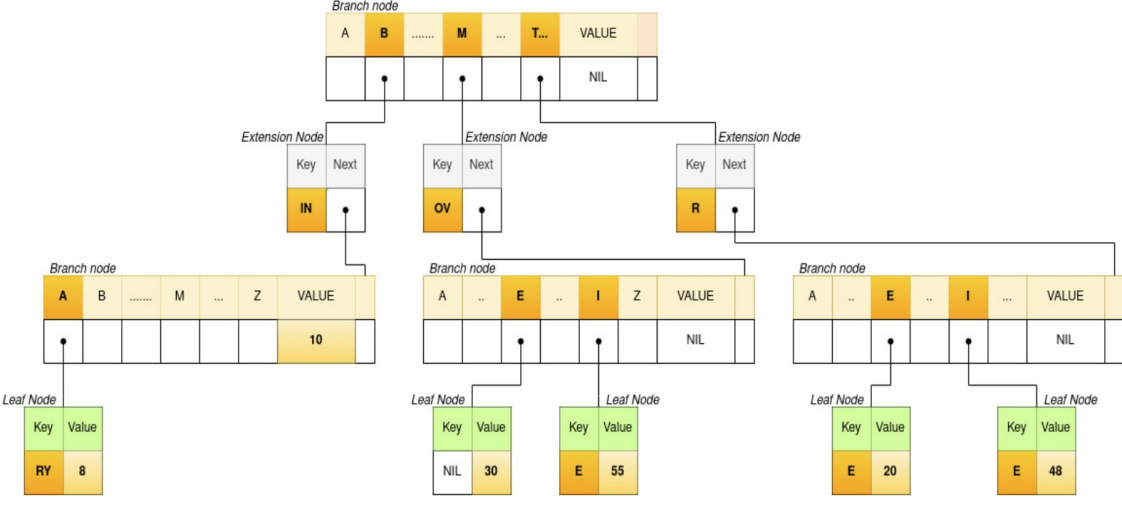
\includegraphics[width=350px]{images/4_Cryptographic_Toolbox/03.png}
    \caption{Patricia trie for key-value pair}
\end{figure}

To make this structure cryptographically secure we pair each node with its hash, so the root becomes a cryptographic fingerprint of the entire data structure and hashes may be used for look-up in a database and to reference child nodes.

\subsubsection{Patricia Merkle Trie in Ethereum}
The ethereum blockchain store the state of the contracts on the blockchain and a set of transactions in blocks.
The state is combination of key-value pair, for example:
\begin{itemize}
    \item key is the address of an account and value is the account balance;
    \item key is the address of a transaction and value is the transferred amount.
\end{itemize}
Of course there are various patricia merkle tries stored in the blobkchain for the various key types.

Nodes of the patricia trie are multi-element, structured records while hash functions is applied to binary string, so we need a way to serialize those structure as byte array, like JSON but more efficient.
The two techniques used by Ethereum are:
\begin{itemize}
    \item Hex prefix encoding (HP): used for encoding/decoding keys (the paths);
    \item Recursive length prefix (RLP): used for encoding/decoding values, corresponding to keys, which may of course be structured values.
\end{itemize}

